\documentclass[10pt,twocolumn,twoside]{gsajnl}
% Use the documentclass option 'lineno' to view line numbers

\usepackage{geometry}
\usepackage{amsmath}
\usepackage{epstopdf}
\usepackage{graphicx}
\usepackage{hyperref}
\usepackage{smartdiagram}  
\usepackage{booktabs}
\usepackage{subfigure}
\usepackage{xcolor}
\usepackage{color, soul}
\usepackage{tabularx}
\usepackage{tikz}
\usepackage[edges]{forest}
\DeclareUnicodeCharacter{2212}{-}
\usepackage{comment}

\usetikzlibrary{shadows.blur}
\usetikzlibrary{arrows,shapes,positioning,shadows,trees}
\tikzset{
  basic/.style  = {draw, text width=2cm, drop shadow, font=\sffamily, rectangle},
  root/.style   = {basic, rounded corners=2pt, thin, align=center,
                   fill=green!30},
  level 2/.style = {basic, rounded corners=6pt, thin,align=center, fill=green!60,
                   text width=8em},
  level 3/.style = {basic, thin, align=left, fill=pink!60, text width=6.5em}
}
\graphicspath{ {./Figures/} }
\everymath{\displaystyle}

\articletype{inv} % article type
% {inv} Investigation
% {gs} Genomic Selection
% {goi} Genetics of Immunity
% {gos} Genetics of Sex
% {mp} Multiparental Populations

\runningtitle{DNA as a digital storage device} % For use in the footer
\runningauthor{FirstAuthorLastname \textit{et al.}}

\title{DNA digital data storage: A review of current methods}

\author[1]{Paria Tahan}
\author[2]{Piermarco Giustini}


\affil[1]{paria.tahan@studenti.unipd.it}
\affil[2]{piermarco.giustini@studenti.unipd.it}


% Use the \equalcontrib command to mark authors with equal
% contributions, using the relevant superscript numbers
%\equalcontrib{1} 
%\equalcontrib{2}

%\correspondingauthoraffiliation[$\ast$]{Corresponding author: Please insert the affiliation correspondence address and email for the corresponding author. The corresponding author should be marked with the relevant number in the author list, as shown in the example.}

\begin{abstract}
Various research into digital data storage methods has led to methods of storing data in DNA strands that satisfy the exponentially growing demand for information storage. In addition to being a natural resource, DNA is an energy-efficient way to store genetic information. Following an explanation of some prerequisites in encoding methods and fundamental theories plus a brief history of the essence of data and the challenges in storing data, we review some of the current and most commonly used methods for embedding data into DNA. Methods will be evaluated via Shannon metrics, which define an approach's effectiveness theoretically.
\end{abstract}

\keywords{Digital Data; DNA Storage; Encoding; Error Correction}

% \dates{\rec{xx xx, xxxx} \acc{xx xx, xxxx}}

\begin{document}

\maketitle

\thispagestyle{firststyle}
%\slugnote I can use this to check all the line that we have wrote
%\firstpagefootnote
\vspace{-10pt}% Only used for adjusting extra space in the left column of the first page


\section{INTRODUCTION}
Having access to so much data in this high-tech era makes the choice on what to act upon or ignore difficult (e.g. more than 12 trillion hours spent online, a monumental milestone in internet adoption, and new records for social media use) \cite{datareportal}.

Automation, machine learning, big data, and artificial intelligence tools have not helped much in that, they have made the process more complicated, which results in a feeling of overwhelm \cite{alliance2021preserving}.

Big data's severe effects can be mitigated by examining the factors that affect it and the data explosion itself. Overall, the first factor in solving this challenge and trying to make it less critical is learning more about the essence of data through the study and the use of its nature and frequency. By and large, we need to save data and it evolves several different approaches to overcome this issue. 

The traditional methods such as CDs, DVDs, flash drivers, and so on can store around 200 GB/$in^2$ data but are not cost-worthy since they occupy a large number of physical storage \cite{wang2019high}. On the other hand, data should maintain and the above methods cannot last long because taps, disks, and other traditional media decay rapidly, in that they can only store data for a short period of time. One of the state-of-the-art techniques is storing digital data in Deoxyribonucleic acid (DNA). We can summarize this technique in one sentence: "The process of encoding and decoding of binary data to and from the DNA strands" \cite{ceze2019molecular}. Through this process we might lose data means either receiving data that is different from the source data or not receiving it at all. Initially, provided research methods couldn't retrieve more than partial data \cite{church2012next}.

This review paper aims to gather some of the required information which is essential to understanding different DNA digital data storage approaches. We first start with a brief introduction to the state of digital storage. The following section will introduce specifically the DNA storage method, and its challenges followed by an explanation of its pipeline. We outlook to the encoding, considered the most important part of this pipeline and related to our curriculum although we know that other parts such as synthesis and storing are the same vital. 
However, we did not deal with this part of the research due to a lack of knowledge and decided to leave it to biology researchers. In order to assess the proposed methods, we went through information metrics. At last, we briefly talked about the utmost goal of all these researches which are related to economics. This review paper will be finished with the conclusion and suggestion for future work. 
\section{STATE OF DIGITAL STORAGE}
\label{sec:STATE OF DIGITAL STORAGE}
In today's world, the storage industry is facing innovation. It is due to the fact that every year more and more data is generated, which engineers are trying to store in the most efficient way possible.
In fact, the digital industry has made staggering improvements in density, size, and total capacity.
%create an image of HHD scale 
\subsection{A brief history of digital storage}
The first hard drive (HDD) was introduced during the 1950s, costed over \$10 per megabyte and had a capacity of maximum 5 megabytes, while nowadays an image can be larger than 5 megabytes. 
Moving closer to our days, in the 2011 disk represented 70\% of all the bytes of storage shipped. The disk industry’s roadmap was used to predict a consistent 40\%/yr improvement in bit density on disk platters, which has now become a 40\%/yr reduction in cost per bit stored. In recent years the industry has failed to achieve this roadmap target. The current roadmap predicts no more than a 20\%/yr improvement in bit density for the next five years. There are reasons to believe that even this may be optimistic, and also that even if it were to be achieved it might not translate directly into a 20\%/yr drop in cost per bit \cite{rosenthal2012economics}.

\subsection{Kryder's Law}
A spin-off of Moore’s Law (the explaination of Moore's law can be found here) is the Kryder's law \cite{walter2005kryder}. Kryder, the former Seagate executive, predicted that the past trend in computer disk storage density would persist into the future, doubling at an exponential rate. However, he noted that the trend was progressing at a much faster rate than the two year timespan of Moore’s Law. Kryder predicted that by 2020 a 40TB disk drive would cost about \$40.
Nevertheless, this has still not been achieved. In fact, in December 2020 Seagate had started to ship 20TB HDD with forecasts of a 50TB model to be made available in 2026 (Figure\ref{fig:my_label1}).
\begin{figure}[ht]
    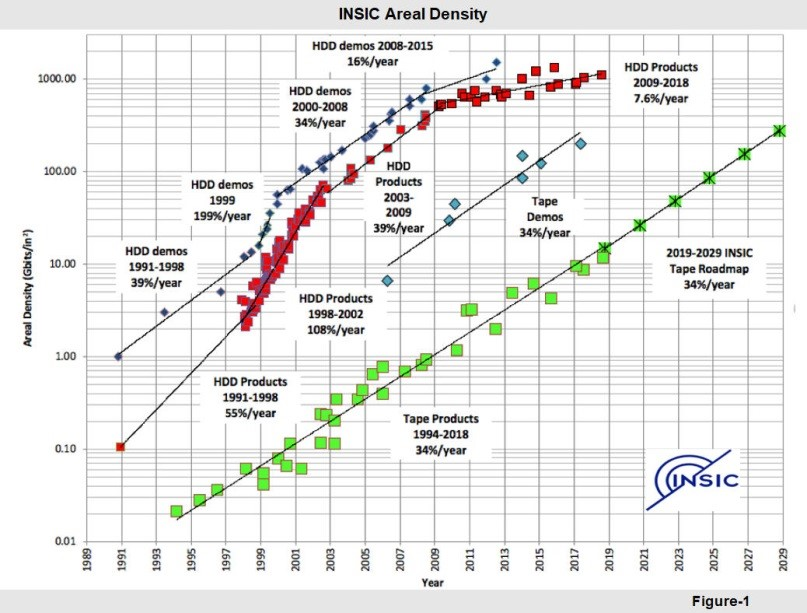
\includegraphics[width=\linewidth]{Figures/LTO-chart.jpg}
    \caption{Caption}
    \centering
    \label{fig:my_label1}
\end{figure}
\subsection{Storage maintenance and replacement}
To link to the previous paragraph, HHD device has short lifespan: almost from 3 up to 5 years before the need to replace it. Data stored in any modern storage devices are periodically re-written onto new generations of devices as well in order to ensure continued access and to provide a better user experience.
Notwithstanding, not all kind of data needs this continuous accessing (better explanation in the two next paragraphs), hence rewriting periodically this data and updating the storage device have higher costs during the time. Consequently a lot of companies are pushing experts to create new kind of long-term storage devices.

\subsection{Energy consumption of digital storage device}    Some studies done in the USA in 2006 indicates that data centers consumed almost 1.5\% of the total energy, this is estimated to be the consumption of 5.8 million average people in the United States for an amount of 4.5 billion\$ . Furthermore, the electricity used by the nation’s servers and data centers in 2006 was more than doubled the electricity that have been consumed in 2000 \cite{shehabi2016united}. Further studies comparing various forecasts show the possible future development of energy consumption.\
In the “best-case scenario” the energy consumption of data centers can remain constant during the time or at least increase slightly. (Figure\ref{fig:my_label2}). Anyway, since Moore's general Law, as said before, cannot be applied and the performance of the data centers increases significantly, annual energy consumption could increase up to 3,000 billion kWh/a. As a consequence, the consumption of data centers will double by 2030 compared to today \cite{hintemann2019energy}.
It is possible to see this trend in the figure below\ref{fig:my_label2})

\begin{figure}[ht]
    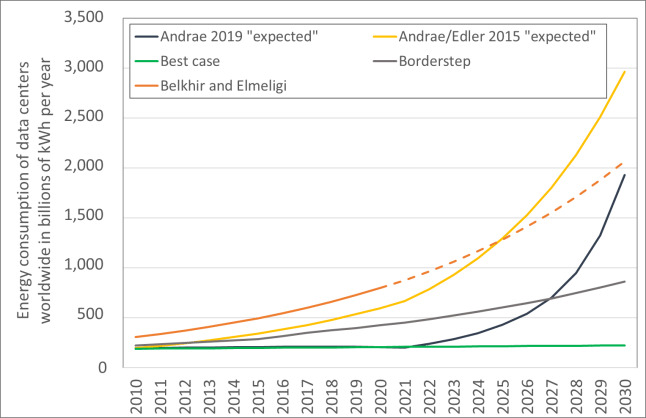
\includegraphics[width=\linewidth]{Figures/Energy-consumption-of-servers-and-data-centers-worldwide-forecasts-to-2030-A-comparison.jpg}
    \centering
    \caption{\cite{inproceedings}}
    \label{fig:my_label2}
\end{figure}

\subsection{Hot-data vs Cold-data}
Storage can be divided into 2 huge different categories: hot data and cold data.
Hot data are data accessed frequently. They are stored in high-performance devices, such as RAM, SSD, and cache, that need frequent access in order to write and read on the memory and need a high temperature to work in the best possible way. A well-known example may be computers whose components exceed 20 Celsius degrees in temperature up to 80.

On the other side, cold data are data accessed less frequently, consequently, they need less heat. Most of the time they are stored on tape + HDD, which may be seen as a huge waste of space and energy consumption.

Such division is fundamental since in recent years a trend is represented by the fast growth of the amount of cold data compared with hot data, this is mainly due to the fact people need to store more data for a longer time. Moreover, it is common that less than 1\% of this data is accessed more than 90-120 days after its creation. 

\section{DNA STORAGE: A COLOSSAL PROBLEM}

\par Having access to so much data in this high-tech era makes it difficult to choose what to act upon or ignore (e.g. more than 12 trillion hours spent online, a monumental milestone in internet adoption, and new records for social media use) \cite{datareportal}.
\par Automation, machine learning, big data, and artificial intelligence tools haven't helped much either. As a result, they have made the process more complicated, which results in a feeling of overwhelm \cite{alliance2021preserving}.
\par Big data's severe effects can be mitigated by examining the factors affecting it and the data explosion itself. In this section we will focus on analyzing hyperscale data needs and potential growth.

\subsection{Amount of Data}
\textbf{TODO} we need to talk about data!
\begin{comment}
\begin{table*}
\centering
\caption{Timeline of the papers used in this survey which worked on \textbf{digital data storage with DNA}}
\begin{tableminipage}{\textwidth}
\begin{tabularx}{\textwidth}{@{}XXXX@{}}
\hline
{\bf Case Study} & {\bf inf capacity} & {\bf Amount of Data} & {\bf Encoding} \footnote{if we need footnote} \\
\hline
\cite{church2012next} & 2012 & 0.65 MB & Physical Redundancy\\
\cite{organick2018random} & 1.81 bits/character & 200.2 MB & Logical Redundancy\\
\cite{grass2015robust} & 2015 & 0.083 MB & Logical Redundancy\\
\cite{bornholt2016dna} & 2016 & 0.151 MB & Logical Redundancy\\
\cite{tabatabaei2015rewritable} & 2015 & 0.017 MB & Logical Redundancy\\
\cite{erlich2017dna} & 1.57 bits/character & 2.15 MB & Logical Redundancy\\
\cite{goldman2013towards} & 2013 & 0.739 MB & Logical Redundancy\\
2018 degenerate & 3.37 bits/character & gg & gg\\
\hline
\end{tabularx}
  \label{tab:shape-functions}
\end{tableminipage}
\end{table*}
\end{comment}
\begin{figure*}[h!]
    \centering
    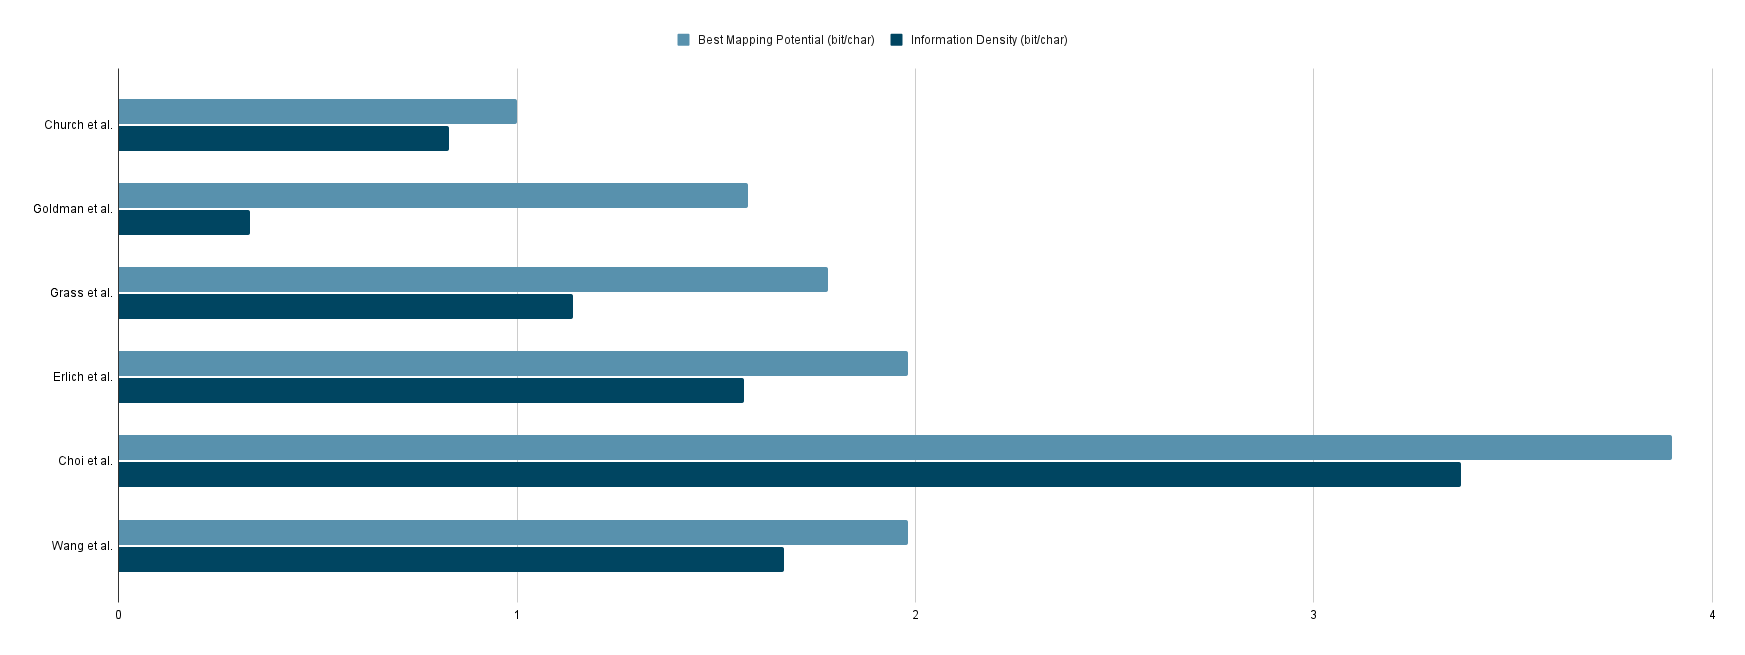
\includegraphics[width = \textwidth]{Figures/shennon chart .png}
    \caption{In this figure, it is possible to see the comparison between the theoretical limit expressed with the Shannon in-
formation and what actually the best papers in the field have managed to achieve. Although the best seems absolutely
the one carried out on the degenerative bases as it reaches excellent values of encoded information. In truth, it is better
to note the difference between the two graphs as the best papers are those that manage to thin the difference between
the theoretical bound and the one actually achieved during the drafting of the experiments.}
    \label{fig:my_label3}
\end{figure*}

\section{DNA Synthesis }
The step after the encoding of the information is one of the most difficult, and it is the one that today creates a good part of the problems, that is the synthesis of DNA, in short, it will be explained what it is and how roughly how it works without going into too much detail.
First, the oligonucleotides are chemically synthesized by creating building blocks their name is nucleoside phosphoramidites. One phosphoramidite is added once per time, the 5' hydroxyl group is deprotected and a new base is added and so on.\\
Nevertheless, due to the fact that is a chemical process, several incorrect interactions occur and this lead to the creation of defective products. 
Furthermore, the longer the oligonucleotide sequence that is being synthesized, the more errors incomes, thus it is better to use this process only for short sequences of nucleotides, but in our case, we would need to create long sequences and this is an important constraint that in future applications will have to be overcome. \\
The current practical limit of this technique is around 200 bp (base pairs) for an oligonucleotide. Meanwhile, a large number of oligos can be synthesized in parallel on gene chips, but for optimal performance in subsequent gene synthesis procedures, they should be prepared individually and on larger scales \cite{wiki:Artificial_gene_synthesis}.

\section{DATA TO DNA: THE DIGITAL DATA PIPELINE }
A vast amount of digital data makes the development of alternative storage methods essential. In the case of DNA-based data storage, the binary data of 0 and 1 is converted into the quaternary encoding nucleotides A, C, G, and T, synthesized, and stored \cite{choi2019high}.
\par Using DNA storage might be an appealing concept because of the following advantages that we have already deeply discussed: a natural genetic information density of petabytes per gram and a durable storage system capable of lasting for centuries without any energy input make DNA storage a stable, resource-efficient and sustainable data storage solution \cite{dong2020dna}.

The DNA storage method is formed by six phases: Coding, Synthesis, Storage, Retrieval, Sequencing, and Decoding. In this review paper, all the phases and their relative methods will be discussed, and a brief comparison among them will be provided.

\begin{center}
\smartdiagramset{priority arrow width=2cm,
priority arrow height advance=2.25cm,
priority arrow head extend=0.3cm}
\smartdiagram[priority descriptive diagram]{Encoding,Synthesis,Storage,Retrieval,Sequencing,Decoding}
\end{center}
\subsection{where the errors occur}
DNA synthesis and sequencing are error-prone. Several papers on DNA data storage report errors of approximately 1\% per base per position28,31,32. More precisely, for a given position in a DNA strand, when synthesized and sequenced back, approximately 1\% of the reads will have an error in that position. 

\section{ENCODING}

Encoding is the process of using a code in order to modify original data into a required form for an external project, in our case to store data in a DNA molecule.\
Anyway, to have a general overview of this process, it is important to introduce the most general case code used for converting characters, which is the Standard Code for Information Interchange (ASCII), the most commonly used encoding scheme for files, where a unique number is assigned to some characters. ASCII contains 2 different types of characters: printable and nonprintable, such as symbols, punctuation marks, numbers, and uppercase and lowercase letters. Encoding is also used to re-size the audio and video files. \

Furthermore, encoding should not be confused with encryption, which hides content. Both techniques are used extensively in the networking, software programming, wireless communication and storage fields.


\subsection{what is error encoding codes}
The results of mathematical manipulation of data to correct errors inserted in the data as bits are stored, transmitted, and so on. The process typically involves computing a summary of the data and storing and/or transmitting it with other data and using the redundant information to correct errors generated. An inner code refers to coding within a single strand to correct local errors. An outer code instead refers to whole new additional strands that deal with errors and which are not covered by inner codes, an example may be erasures.
Erasures
The removal of writing recorded material or data.\

In a nutshell, reliable data storage and retrieval need error correction methods for all types of media (and communication channels such as radios). In this case, it is possible to mention a whole field of computer science called information theory, or coding theory, that focuses on developing coding schemes able to deliver digital data reliably over noisy media and communication channels. One especially interesting aspect of DNA is that, unlike other storage channels, characterized only by substitution errors, DNA channels can also manifest base insertions and deletions, which makes decoding more challenging.\

Error correction codes reduce by adding redundant information, which increases the probability of the original information to be retrieved even in the presence of errors or missing data. The more redundancy, the more tolerant of errors (or losses) the resulting storage process will be. Redundancy can be of two basic types. Physical redundancy comes from having many physical copies of a given DNA sequence. Logical redundancy comes from embedding additional information when encoding data in the DNA sequences.

These sequences may go through a logical ‘exclusive-or’ operation with a pseudo-random number generated from a known seed to ensure that DNA strands are dissimilar, and then redundancy is added via codes, such as Reed–Solomon codes, for error correction purposes. Different encoders may then use different rules to convert bits to sequences. A common conversion rule is to avoid repeated bases (homopolymers) and to add primer target sites on both ends.

The first modern error-correcting codes appeared in the 1940s. Generally, all error-correcting codes add redundancy to the original data to be stored or transmitted over a channel. Receivers can use this extra redundant data to check whether the received message is consistent and, if it is not, to potentially reconstruct the original data. The amount of redundant data to be added can vary depending on the noise profile of a channel, on the code used, and on the desired probability of successful decoding.




% \begin{figure*}
% \centering
% \caption{An illustration of a simple delete operation. \label{fig:simple}}

% \forestset{parent color/.style args={#1}{
%     {fill=#1},
%     for tree={fill/.wrap pgfmath arg={#1!##1}{1/level()*80},draw=#1!80!darkgray}},
%     root color/.style args={#1}{fill={{#1!60!gray!25},draw=#1!80!darkgray}}
% }
% \begin{forest}
% forked edges,
% for tree={draw,rounded corners,align=center,edge={-latex},fill=white,blur shadow}
% [Digital Data Storage Using DNA Methods Taxonomy,root color={teal}
%  [Storing Without Compression,parent color={purple}]
%  [Storing With Compression,parent color={olive}
%   [Using Error Correction,parent color={lime}
%   [Linear Block \\ Code]
%   [Reed-Solomon \\ Code]
%   [Fountain \\ Code]
%   [Using \\ Silica Spheres]
%   ]
%   [Without Using Error Correction,parent color={gray}
%   [Directly \\ Encoding]
%   [Using \\ HTML]
%   ]
%  ]
% ]
% \end{forest}
% \end{figure*}

%%%%%%%%%%%%%%%%%%%%%%%%%%%%%%%%%%%%%%%%%%%%%%%%%%%%%%%%%%%%%%%%%%%%%%%%%%%%%%%%%%%%%%%%%%%%%%%
\subsection{Shannon Information as a metrics}
DNA storage is a communication channel that receives data by sequencing the oligos\footnote{Oligonucleotide}. Anyway, the channels are noisy due to various steps of DNA encoding, such as DNA synthesis imperfection, PCR dropout, stutter noise, sequencing errors, and even degradation of DNA molecules over time, known also as experimental factors.
These kinds of errors are really different from the binary counterpart, where the noise is identical and independently distributed, on the contrary, the DNA error pattern heavily depends on the input sequences.
Anyway, a lot of previous studies on the error pattern show that the running homopolymer and the GC content are the major determinants of synthesis and sequencing error.
Shannon provides results about resources needed for optimal coding and error-free communication and helps to measure the quality of DNA storage encoding.
Hereafter there is an explanation of how it works.
According to Shannon exist a general communication system:
\begin{itemize}
    \item A Source $S$, which generates the message.
    \item A Transmitted $T$, which turns the generated massage into a signal to be transmitted.
    \item A Channel $CH$, that is, the medium used to transmit the signal from the transmitter to the receiver.
    \item A receiver $R$, which reconstructs the message from the signal.
    \item A destination $D$, which receives the message.
\end{itemize}

In the sorce $S$ there is a range of possible state starters $s_{1},..., s_{n}$ called $Latters$, and their respective prob are given by $p(s_{1}),...,p(s_{n})$ .
So the amount of information generated is defined as:
\begin{center}
$I(s_{i}) = \log(1/p(s_{i})) = - \log(p(s_{i}))$
\end{center}
Since $S$ produces sequences of state called messages, so the full entropy of the source S is defined as using the minus form:
\begin{center}
$ H(S) = - \sum_{i = 1}^{n} \log(p(s_{i}))$
\end{center}
Analogously we have the same value for the destination $D$ so y $d_{1},..., d_{m}$ the range of destination reached, with the respectively probabilities $p(d_{1}),...,p(s_{m})$. The amount of information received at the destination is measured as:
\begin{center}
$I(d_{j}) = \log(1/p(d_{j})) = - \log(p(s_{j}))$
\end{center}
and its $entropy$ it s defined:
\begin{center}
$ H(D) = - \sum_{j = 1}^{m} C$
\end{center}
Furthermore, looking at the previous formulas, it is possible to notice that a logarithmic function is used, because mathematically the log function is more suitable due to many limiting operations in log which are easier. Moreover, by choosing a base 2, the resulting amount of information obtained is called $bit$ that is the UNIT in digital storage.
Deeply on the details, now a bit is the amount of information obtained on two equally likely specified alternatives.
The image above shows the relation between the source information $H(S)$ and the destination $H(D)$:\\
\begin{itemize}
    \item $H(S;D)=H(S) \cap H(D)$ is the $mutual information$ the amount of information generated by the source and correctly received by the destination
    \item $E=H(S) \backslash H(S;D)$ is the $equivocation$ the amount of information generated by source but not received by destination.
    \item $N=H(D) \backslash H(S;D)$is the $noise$ the information received by the destination but not generated by the source.
\end{itemize}
In addition, Shannon's information does not depend only on the information sent and received but it is also necessary to take into account the $CH$ crossed transmission channel. In the case analyzed in this paper, the channel is the synthesized DNA molecule.
The introduction of the communication channel brings immediately the possibility of errors in the process of transmission.
As a conclusion, it is possible to take into account those errors by defining the matrix $[p(d_{j}\backslash s_{i})]$ where $p(d_{j}\backslash s_{i})$ is the conditional probability of the $d_{j}$ in the destination. As a consequence, it is possible to compute N and E in the following way:
\begin{center}
$ N = \sum_{j = 1}^{m} p(s_{i}) \sum_{i = 1}^{n} (p(d_{j}/s_{i})) \log(1/p(d_{j}/s_{i}))$
\end{center}
\begin{center}
$ E = \sum_{j = 1}^{m} p(d_{j}) \sum_{i = 1}^{n} (p(s_{i}/d_{j})) \log(1/p(s_{i}/d_{j}))$
\end{center}
where $p(s_{i}/d_{j}) = \frac{p(d_{j}/s_{i})p(s_{i})}{p(d_{j})}$.\\
The $CH$ $capacity$ is defined as: 
\begin{center}
    $C = max_{p(s_{i})}{H(S;D)}$
\end{center}
The maximum is taken all over the distribution $p(s_{i})$ from the source, instead, $C$ measures the larger amount of information that can pass over the communication channel $CH$.
For summaries Shannon provides two important theorems to measure information transmission:
\begin{itemize}
    \item $First Theorem$ or $Noiseless-Channel Coding$, in order to have a sufficiently long message, the value of $entropy (H(S))$ should be equal to the average number of symbols necessary to encode one letter of the source (GTAC) by using an ideal code.
    \item $Second Theorem$ or $Noisy-Channel Coding$ says that the channel capacity is equal to the maximum rate at which the information is sent and recovered at the destination with a vanishingly low prob error.
   \end{itemize}
Further details on Shannon can be found \cite{lombardi2016shannon}.
\subsection{Definition of information capacity}
By skipping some math behind Shannon and the definition of the information capacity, it is possible to give an easier explanation of the term ‘Bytes per bases‘: "The input information in bits divided by the number of synthesized DNA nucleotides."\
Even though the unit for the term is slightly different in the literature, the parameter is used to determine how much data can be encoded in the DNA sequence, before the synthesis of the DNA itself. Therefore, it is a value that can intuitively convey the performance of data to the DNA by encoding algorithm.
\begin{center}
    $\frac{\log_{2}(K)}{l} bits/character $
\end{center}
$K$ $=$ $Numbers$ $of$ $codon$\\
$l$ $=$ $Numbers$ $of$ $base$ $per$ $codon$
\\Example of usage:\\
to use 15 basis $"A,T,G,C,Y......"$ so 750 codons are generated $(K)$ $ATC,ATY,ATG ....$ in 3-base-codons $(l)$ are generated.\\
From this term should be multiplied other factor terms that depend on the encoding strategies and the error correction coding used.
In 
% ?!
%%%%%%%%%%%%%%%%%%%%%%%%%%%%%%%%%%%%%%%%%%%%%%%%%%%%%%%%%%%%%%%%%%%%%%%%%%%%%%%%%%%%%%%%%%%%%%%%%%%%%%%%%%%%%%%%%%%%%%%%%%%%%%%%%%%%%%%%%%
\section{Reed-Solomon}
In \cite{grass2015robust} they showed that digital information can be stored on DNA and recovered without errors for considerably longer time frames. They encapsulated the DNA in an inorganic matrix, and employed error-correcting codes to correct storage-related errors. Nucleotides were encapsulated in silica. The original information could be recovered error free, even after treating the DNA in silica at 708C for one week.
\begin{figure*}[h!]
    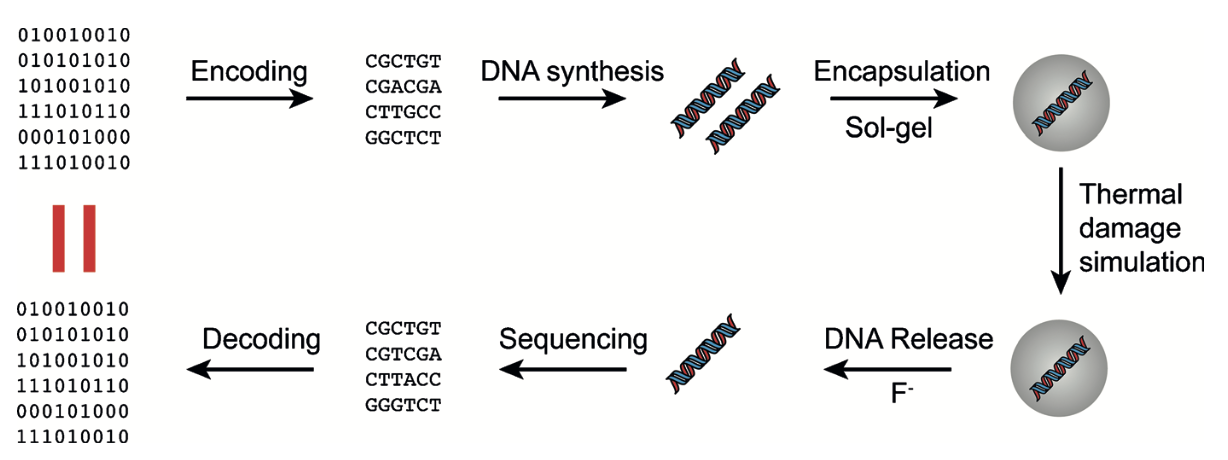
\includegraphics[width=\linewidth]{Figures/Reed-Solomon-Silica.png}
    \caption{Digital information is encoded to DNA and encapsulated within silica spheres. Upon release of the DNA from the spheres by fluoride chemistry, the DNA is read by Illumine sequencing and decoded to recover the original information, even if errors were introduced during the procedures.}
    \centering
    \label{fig:my_label4}
\end{figure*}

The general idea of this case study was as follows: Individual sequences are indexed and two independent error-correcting codes (specifically Reed–Solomon codes) are used in a concatenated fashion.

\begin{figure*}[h!]
    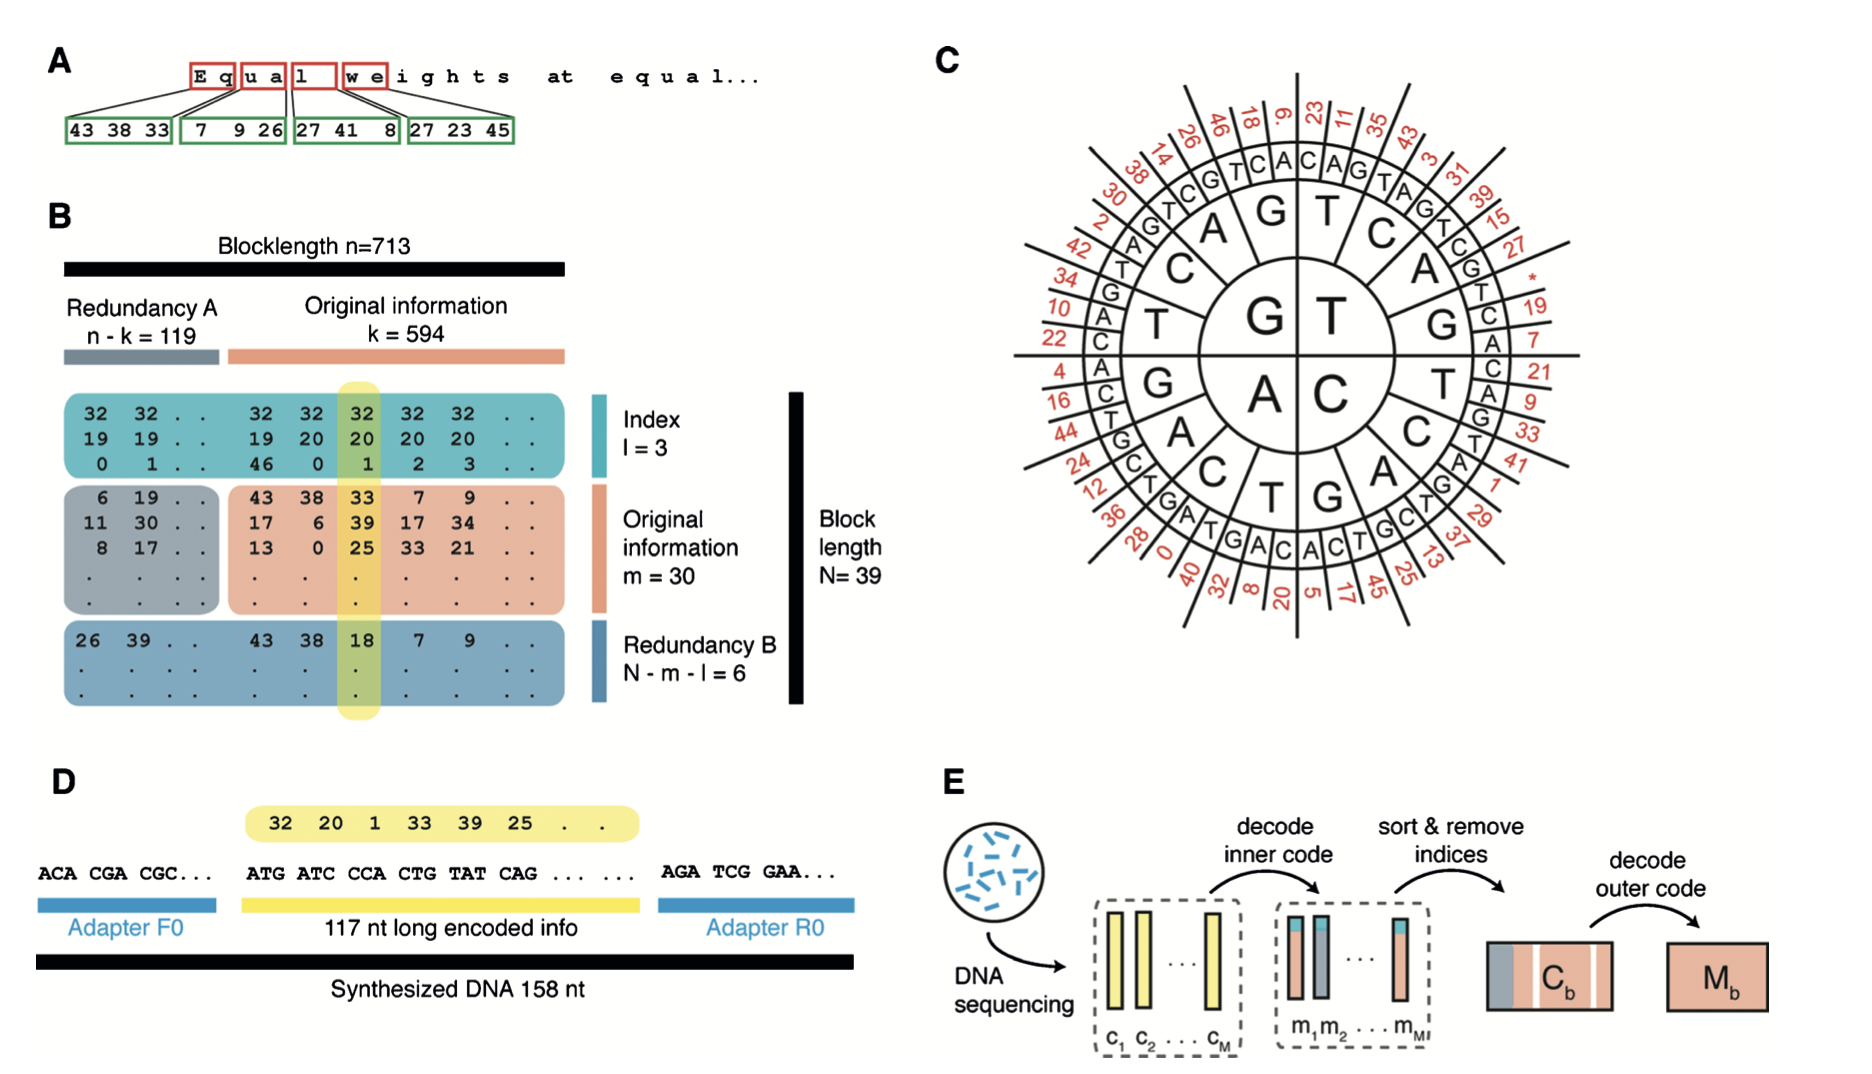
\includegraphics[width=\linewidth]{Figures/reed-solomon-error-correction.png}
    \caption{Encoding text to DNA by Reed–Solomon coding: A) Two letters of a text file (or more general, two bytes of a digital file) are mapped to three elements of the Galois Field of size 47 (GF(47)) by base conversion (2562 to 473). This original information is arranged in blocks of \(594 \times 39\) elements. B) In an outer encoding step Reed–Solomon (RS) codes are employed to add redundancy A to the individual blocks. To each column an index is added and redundancy B is generated using a second (inner) RS encoding step. C) The individual columns are converted into DNA by mapping every element of GF(47) to three nucleotides by utilizing the GF(47)toDNA codon wheel, thereby guaranteeing that no base is repeated more than three times. D) Two constant adapters are added and the resulting sequences of 158 nucleotides are synthesized. E) To recover the original information from the DNA, the read sequences are translated to GF(47) and are decoded by first decoding the inner code (correcting individual base errors), sorting the sequences by means of the index, followed by outer-decoding, which allows the correction of whole sequences and the recovery of completely lost sequences (see the Supporting Information for details on coding and experimental procedures).}
    \centering
   \label{fig:my_label5}
\end{figure*}
%%%%%%%%%%%%%%%%%%%%%%%%%%%%%%%%%%%%%%%%%%%%%%%%%%%%%%%%%%%%%%%%%%%%%%%%%%%%%%%%%%%%%%%%%%%%%

\section{DNA Fountain approach}
A study conducted by Y.Erlich and D.Zenlinki in 2017 has changed the way of coding the information into DNA molecules and in some cases, it was possible to retrieve perfectly the information.
The technique they used is known as DNA Fountain. 
The strategy works with fountains codes which allow reliable and effective unicasting of the information over channels, that are subject to dropouts.
It is possible to divide the technique into 3 parts:
\begin{itemize}
    \item The first step provides for the processing of a binary file into a series of $non-overlapping$ $segment$ of a fixed length, the files then are packed into a single tape-archive file, which is afterward compressed by using a common lossless algorithm. 
    
    \item At this point the $Luby$ $Transform$ $Algorithm$ is applied, it sets the basis and prepares them for the fountain transform. Moreover, it transforms the data into packages called droplets, selecting them by using a special distribution and adding them bitwise together under a binary file.
    The droplets contains two pieces of information:
    
    \begin{itemize}
        \item $data$ $payloads$ that holds the result of the addition procedure.
        
        \item $fixed$ $length$ $seed$, this seed is randomly generated from the distribution mentioned above and this allows the decoder algorithm to infer the identities of segment droplets.
    \end{itemize}
    
    \item Afterwards the algorithm moves to the $screening$ part, where the algorithm translates the binary droplets to a DNA sequence by converting ${00, 01 , 10, 11}$ to ${A, G , G , T}$. Then it screens the sequence, and whether it passes the screening it is considered valid and added to oligos design files, otherwise, it gets discarded.
    It is possible to iterate this step until it is not found a correct amount of valid oligos. 
\end{itemize}
Most importantly, Erlich and Zenlinki have been able to achieve an information density of $1.57bit/nt$ which was a huge improvement from the previous studies that instead achieved a density of a maximum $1.14bit/nt$.

\subsection{Luby Transform Algorithm}
\begin{enumerate}

\item First initialize a $pseudorandom$ number generator $PRNG$ with a seed. The seed is selected by a mathematical rule.
\item The algorithm decides on $d$, the number of segments to package into the droplet. To do this the algorithm calls the PRNG function that draws a random number from a special distribution function (more details in the paper).

\item The algorithm uses again the PRNG to draw d segments but in this case with a uniform distribution and without the replacement of the previous draw.

\item The algorithm performs a bitwise-XOR operation mod 2 on the segments.
\begin{center}
\[ XOR(x,y) =
  \begin{cases}
     0 & \text{if } x = y\\
     1 & \text{if } x \ne y
  \end{cases}
\]
\end{center}
where x and y the bits is the same position but from the different string of bits, example( $0010$ XOR $1010$ = $1000$).

\item Furthermore the algorithm creates a fixed-length index that specifies the binary representation of the seed. For example, if the seed is 1 and the fixed index length is 2bits, the output droplet will be $10$ $+$ $1000$, where 10 is the encoding of 1 in binary $2^{0}$.

\item the user has the option to utilize a regular error correcting code computed on the entire droplet, or a widely used error correction code called Reed-Solomon \cite{erlich2017dna}.
\end{enumerate}


%%%%%%%%%%%%%%%%%%%%%%%%%%%%%%%%%%%%%%%%%%%%%%%%%%%%%%%%%%%%%%%%%%%%%%%%%%%%%%%%%%%%%%%%%%%%%%

\section{Degenerate Basis Approach}
DNA with a degenerate basis is trying to solve a big problem of the maximal information stored inside a sequence of DNA, For example, previous studies try to fix this problem by developing a cheaper synthesis phase, because of the cost of writing (storing the data) is really huge, or at least try to find a better encoding algorithm. However, the most simple and straightforward way is to maximize the amount of data that can be stored per length of the DNA sequence that is designed. 
By looking at the DNA Fountain approach done by Erlich and Dina Zenlinki they were able to have a theoretical information capacity limit of $\log_{2}(4)$ or $2bits/character$.
By the way, if in addition to the standard encoding oligos introduced the degenerate basis, the information capacity of $\log_{2}(number of encoding characters)$ drastically increases, so it reduces the cost of the DNA data storage.
Degenerate bases are stored in the DNA sequence when oligos are grouped together at some specific position in the sequence of the DNA.
\\For example:
\begin{center}
$"AWC"$ where $"A"$ and $"C"$ represent their specific oligos and W represent as said before a mixed pool of $"A"$ and $"T"$. Moreover, it is possible to define 2 types of nucleotides $"AAC"$ and $"ATC$ 
\end{center}
So by using these methods it is possible to achieve a better result in terms of information capacity of $3.37 bits/nt$.
The $Figure 5$ it is presented the structure of the DNA-based data storage used for DNA coding.

\begin{figure*}[h!]
\centering
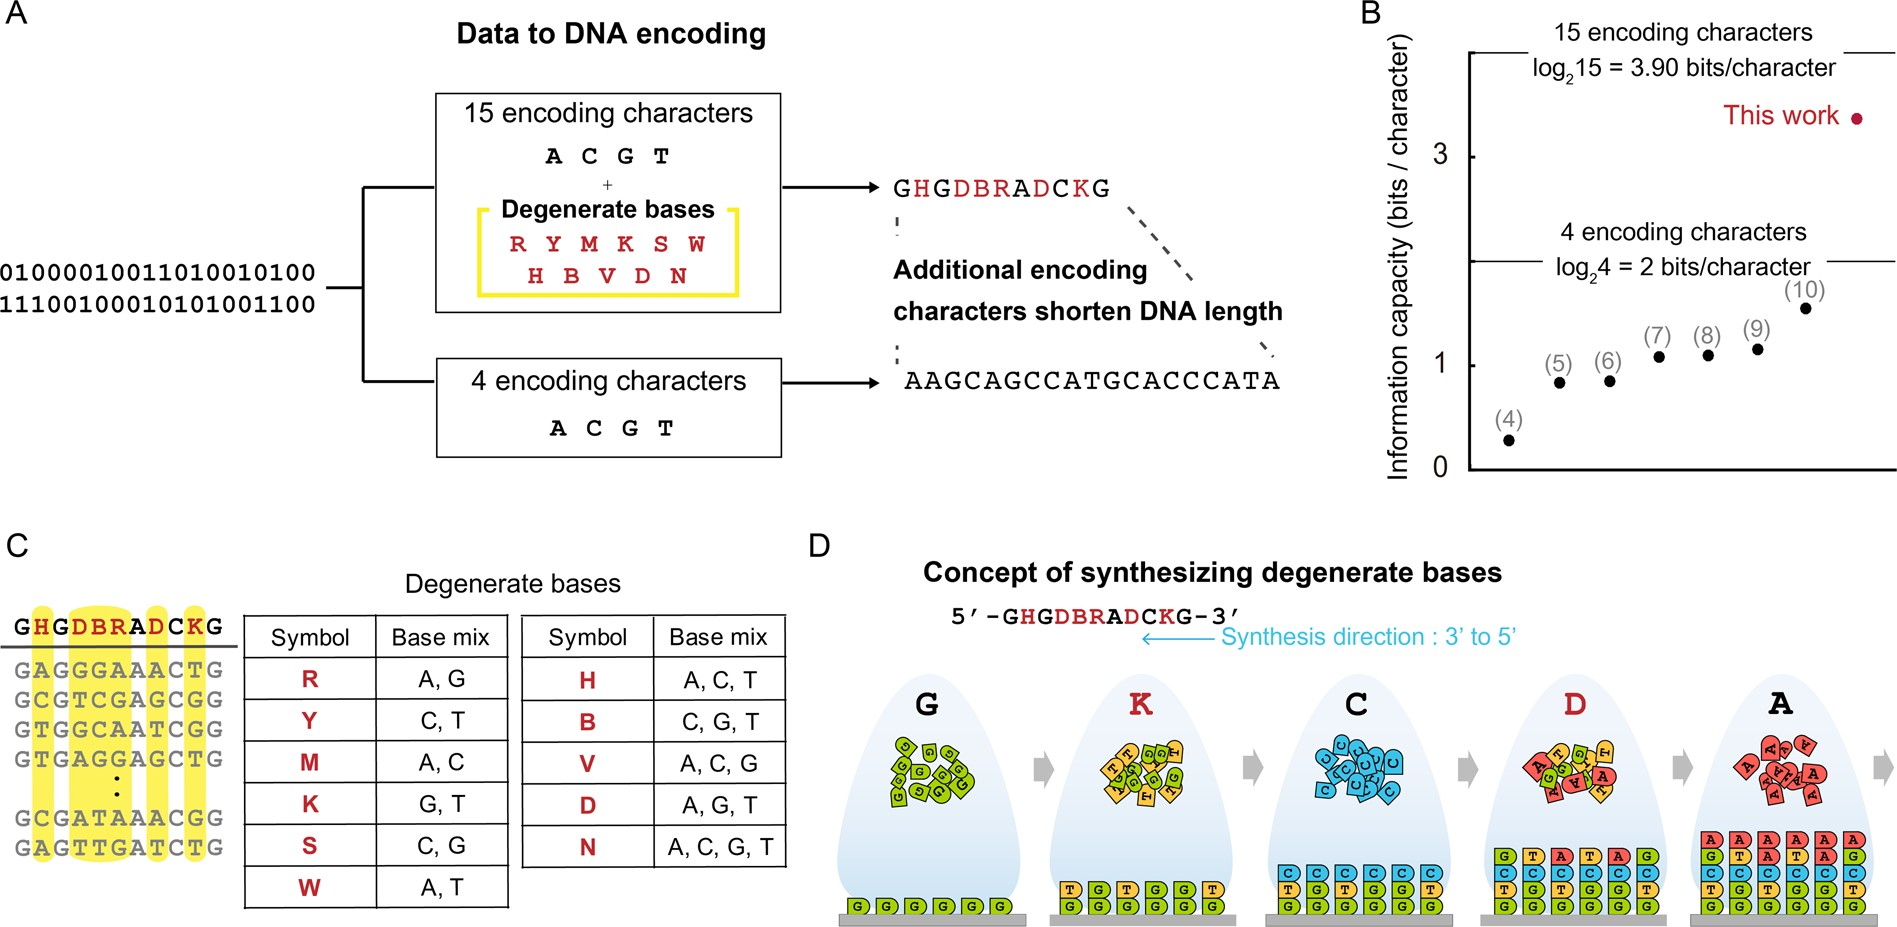
\includegraphics[width=\linewidth]{image degenerate basis.jpg}
\caption{
\\The addition of degenerate bases increased information capacity.\\
(A) Binary data is encoded to DNA sequences comprising not only the 4 traditional encoding characters A, C, G, and T but also 11 additional degenerate bases. But instead, the length of the encoded DNA is shorter than the four-character encoding method. \\
(B) Furthermore the theoretical information capacity is increased from 2 bits/character to 3.9 bits/character. The dots describe the information capacity values in previous research, more precisely the last one refers to the DNA fountain approach that scores the best value.\\ 
(C) A degenerate base represented by an encoding character describes a mixed pool of more than two types of nucleotides, so it is possible to store more information in each oligo.\\
(D) Degenerate bases can be generated by mixing the DNA phosphoramidites during the synthesis procedure.}
\label{fig:my_label6}
\end{figure*}
\begin{figure*}[h!]
\centering
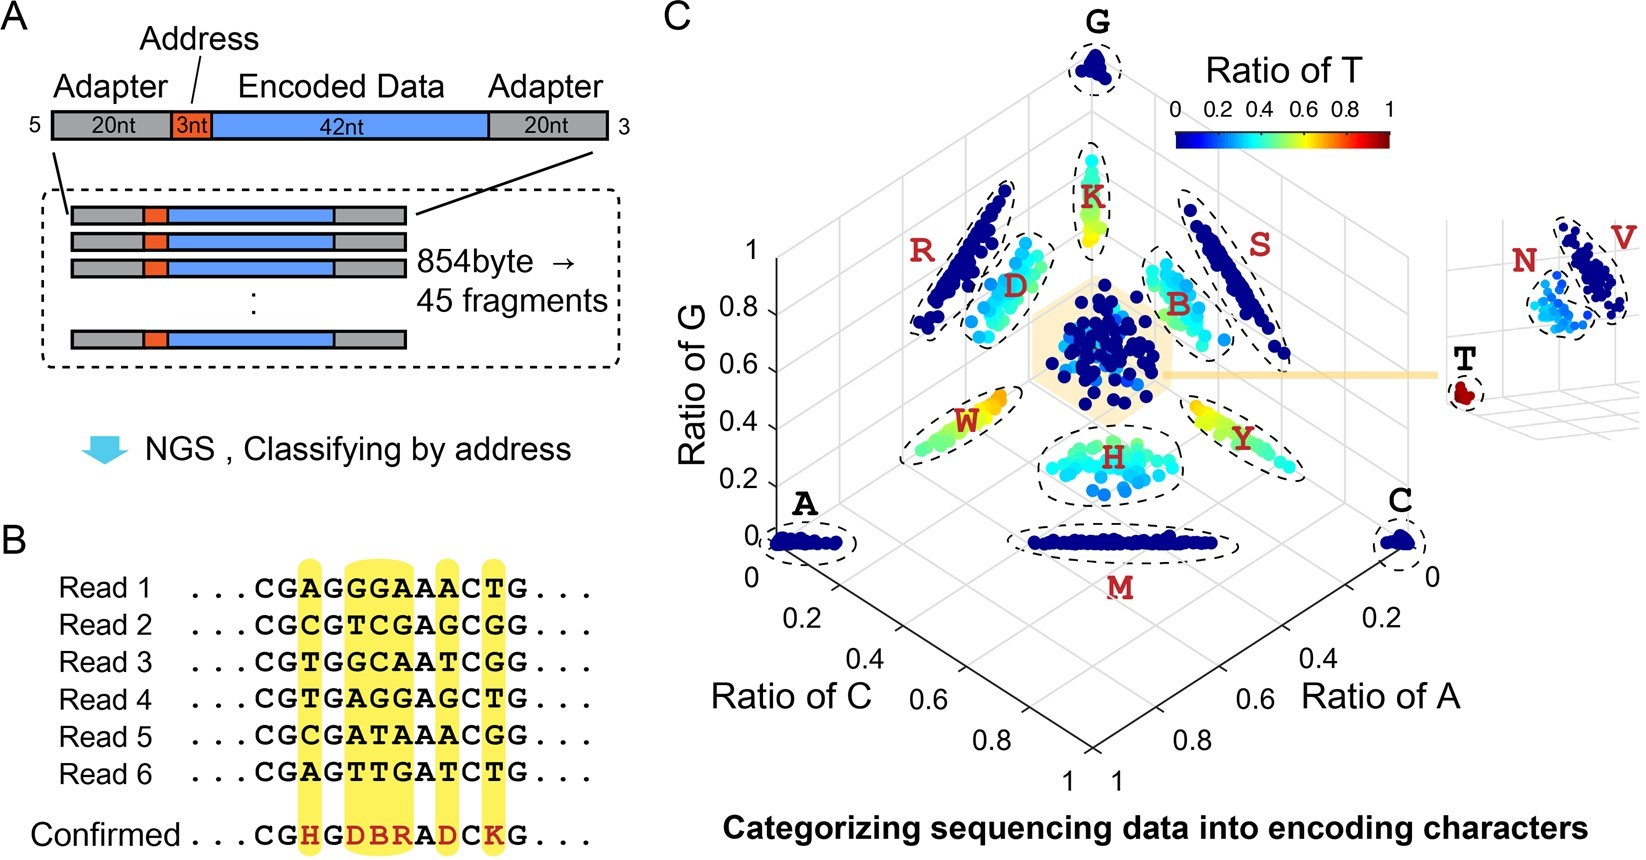
\includegraphics[width=\linewidth]{other on degenerate basis.jpg}
\caption{
\\(A) Design structure of DNA fragments. \\(B) DNA fragments can be analyzed using NGS. After classification by address, degenerate bases can be decoded by examining the distribution of characters in the same position (yellow bar). \\(C) Degenerate bases can be determined from the scatter plot of the ratio of bases in the same position}
\label{fig:my_label7}
\end{figure*}

\section {Variable length oligonucleotides Approach}
The older paper explored finds a lot of problems, in particular, they dealt with two big issues that have to be faced in DNA data storage. \\First, is to design appropriate error correction coding to reach the errors induced from synthesis, storage, sample preparation, and sequencing pipeline.\\
The second deal with the design of a DNA mapping strategy, that convert binary files into DNA sequences under some biochemical constraints.\\
Moreover, by looking at the 2 precedent approach proposed by The DNA Fountain and the addition of the degenerate basis, it is true that really high $bits/nt$ is reached but necessitates higher sequencing improvement and also synthesis techniques for practical usage.
Additionally, this approach does not start from the degenerate basis but it starts from the DNA fountain and tries to improve the solution given by Yaniv Erlich and Dina Zenlinki.\\
To overcome the limitation of DNA fountain, this approach explores another practical common error and really efficient DNA mapping strategy. In particular, the hybrid mapping scheme consists of 2 different mapping methods: 
\begin{itemize}
    \item Interval mapping.
    \item variable-length constraint $VLC$ mapping.
\end{itemize}
they are create to reach the optimal $2bits/nt$ while balance 2 important constraint:
\begin{itemize}
    \item $"GC"$ content.
    \item and $maximum homopolymer run$ limit.
\end{itemize}
Furthermore, a packet-level called $RA$ $code$ is elaborate, low encoding/decoding complexity and high error resilience. Hence, by summing up the $RA$ $code$ and the $hybrid$ $ mapping$ it is possible to reach a robust scheme to store the data inside the DNA.
This approach by the way was able to score the higher density nt information by achieving $1.67bits/nt$ by using these techniques.\\
In the above subsection, we are going to give a general explanation of those tho important components.

\subsection{RA code design}
RA code in the traditional communication system is used to mitigate substitution error income.
In DNA storage cases it is also important to take into account insertion errors and deletion errors. So instead of doing a bit-level $RA$ $coding$, in this paper, it is developed and $RA$ $coding$ packet level.
A large digital file is segmented into packets of the same size. The packets are considered as the source packets which are used to generate the redundant or parity packets using systematic RA code Fig. Also, every packet is incorporated with $CRC$ to detect errors. For 
the packets that pass the $CRC$ check, they are considered correctly recovered while others are dropped. More details are given in the figures.
\subsection{Hybrid mapping scheme}
DNA mapping strategies should be able to map as well as possible the oligos sequences.
Now see how those 2 mapping work:
The interleaved mapping works at approximately optimum mapping potential, almost $1.99 bits/nt$ and the $VLC$ one works as the backup when the interleaved fails to produce valid DNA sequences, the mean of valid is due to the fact the sequences have to satisfy the 2 constraints.
In interleaved mapping the data are mapped to generate a binary sequence, the $GC$ constraint is almost fully satisfied, but it fails the homo polymer run constraint. Any way to solve this problem here is to place the interleaved mapping that scrambles the original order of nucleotide sequence. After doing this step the sequence is tested again if it passes the test, that sequence is considered a valid synthesis, otherwise, it is performed the mapping on the original sequences again.
On the other side, the $VLC$ mapping is inspired by the creation of variable length constrain sequence code, used to encode the data into constraint-satisfying codes. The mapping rules are generated by the following 4 stages:
\begin{enumerate}
    \item considering the constraint of the maximum homopolymer runs, the DNA data storage sequences were generated according to the $FSTD$ diagram Fig.
    \item based on the sequence generated by the $FSTD$, it is possible to deduce the capacity of the homo-polymer constraint, and also establish a minimal set of words whose word contains sequences that satisfy the constraint.
    \item Now by using $Huffman$ coding tree to generate the optimal mapping from the source word set defined before.
    \item the binary sequences generated are encoded according to a change state function, resulting in final oligo sequences that satisfy the constraints.
\end{enumerate}
\newpage
\begin{figure*}[h!]
\centering
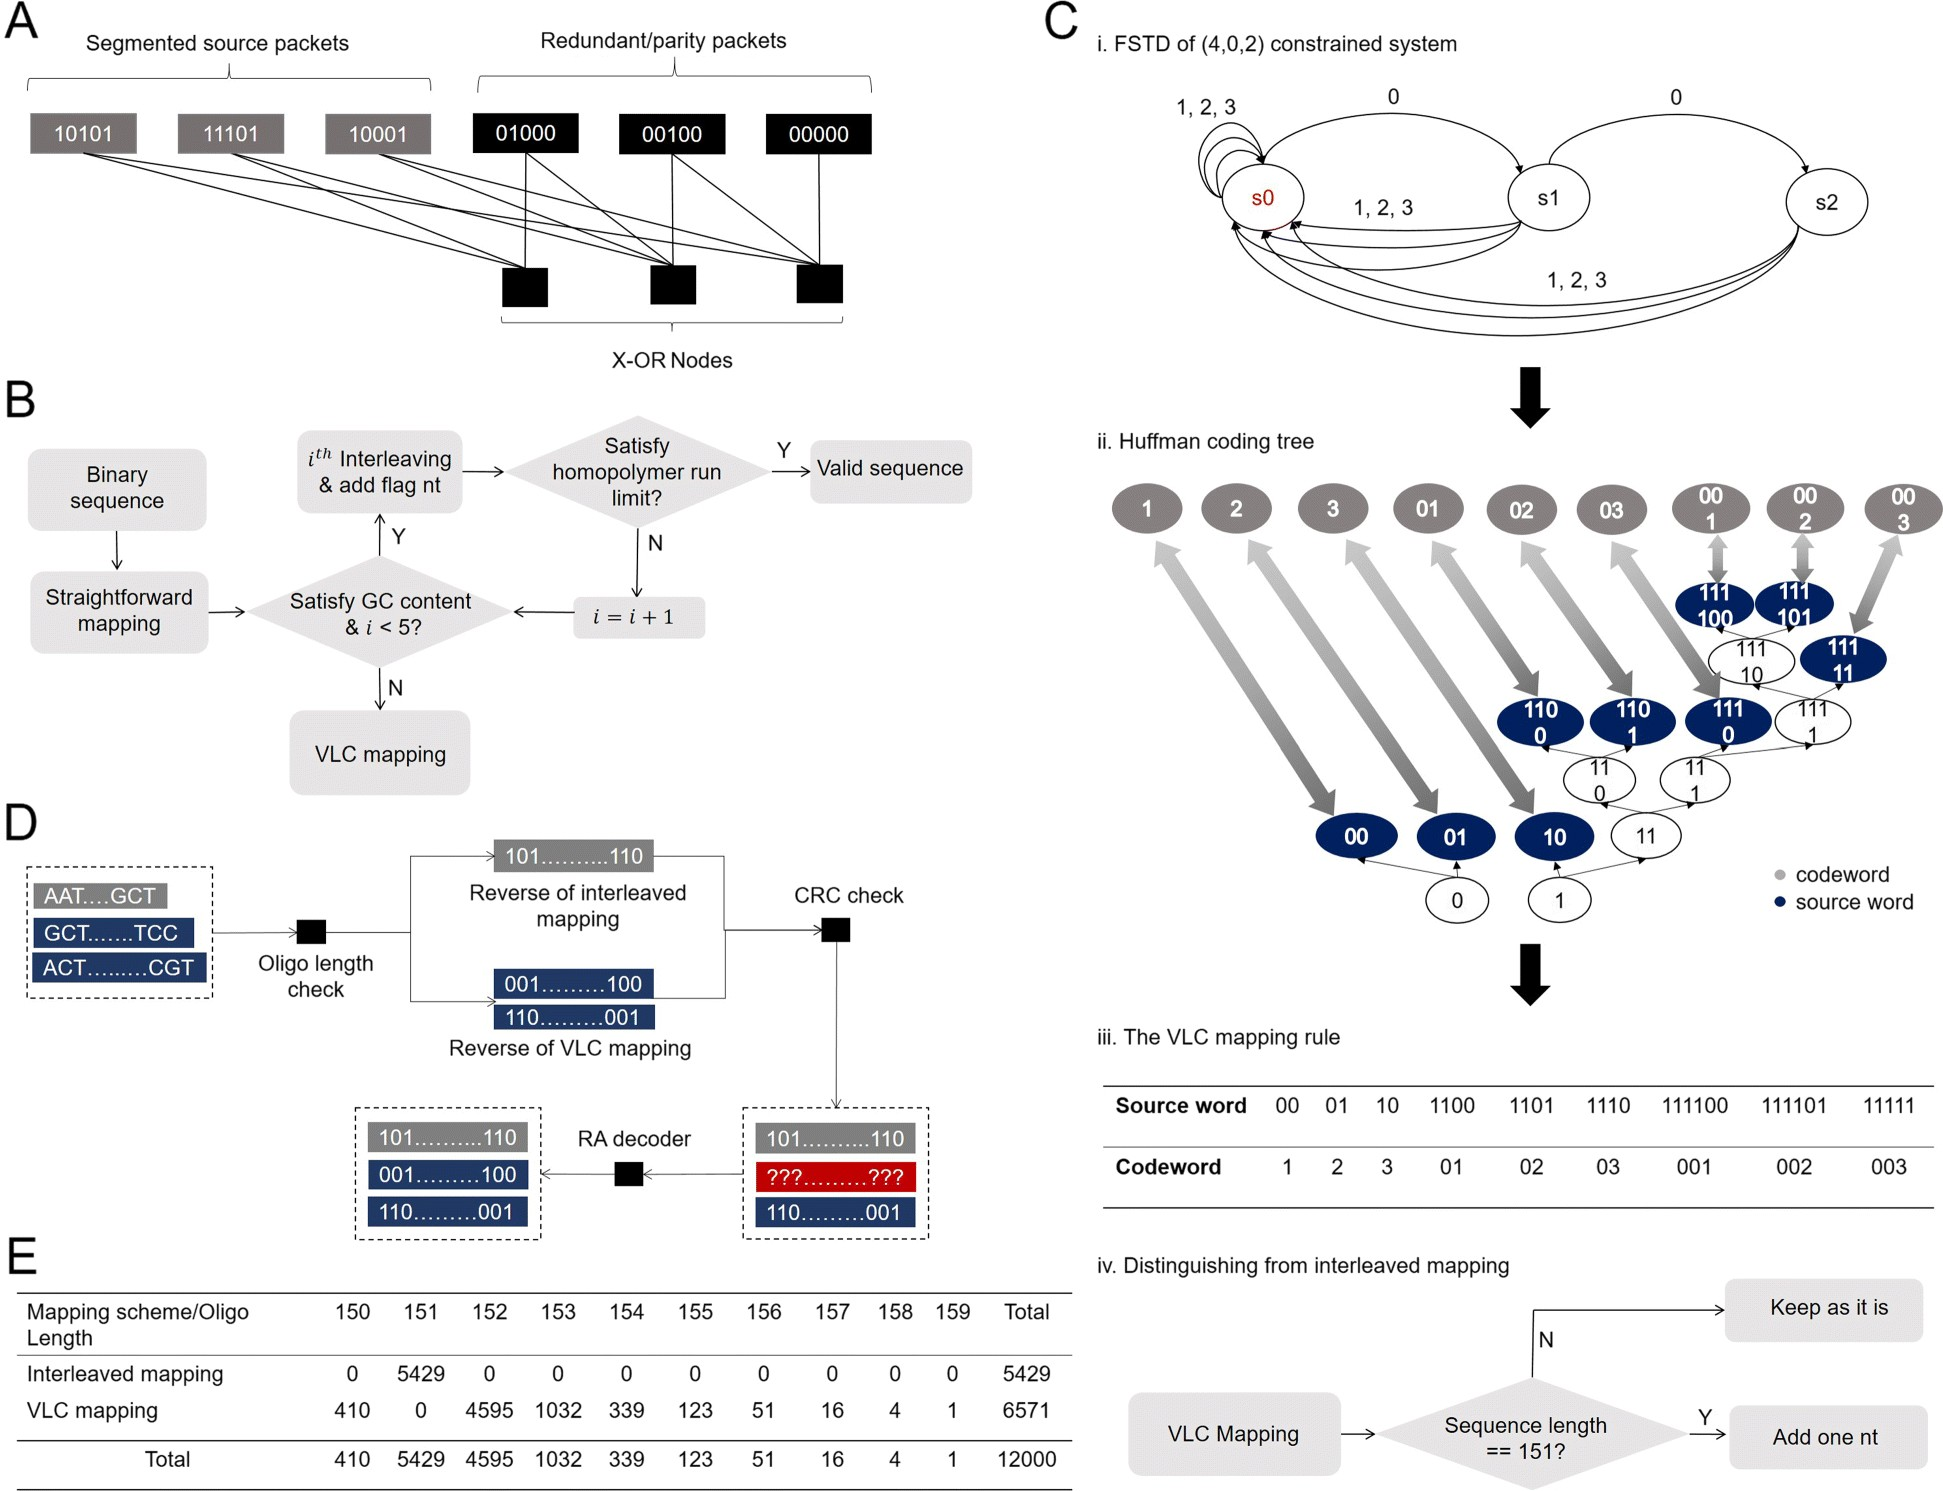
\includegraphics[width=\linewidth]{figure hybrid mapping.jpg}
\caption{The illustration try to give a better explanation of (RA) coding strategies and the hybrid mapping taken from the \cite{wang2019high} that explain in correct words all the process behind.
\\(A) An example of rate 12 packet level RA code with 3 source packets. A ith parity packet at position i is generated by bit-wise mod-2 sum of the (i−1)th parity packet and the source packets that are connected to the ith X-OR node. 
\\(B) The flow chart of the hybrid mapping. Each binary sequence is initially mapped via binary-to-quaternary mapping. With one of interleaving patterns, the interleaved sequence with the flag nucleotide appending at the end might pass the screening test where GC content and homopolymer are checked, outputting a valid sequence. Otherwise, the original binary sequence will be sent to the variable-length constrained (VLC) mapping.
\\(C. i) The $FSTD$ of a (4, 0, 2) constrained DNA storage system, where 0, 1, 2, and 3 represent four transition symbols that indicate the transitions among four nucleotide alphabets, and s0, s1 and s2 represent three different states that record the length of consecutive 0’s (no transition) in the output (4, 0, 2) constrained sequences. 
\\(C. ii) The generation of a $Huffman coding tree$. The Huffman coding tree optimizes the code rate by aligning the source word with high occurrence possibility to the codeword with short length and verse vice. (C. iii) The VLC mapping rule. The alignment of Huffman coding tree generates a look-up table between variable-length source words and variable-length transition codewords. \\(C. iv) The strategy for enabling the decoder to distinguish two mappings via the length of received DNA sequence. 
\\(D) The flow chart of the decoder. The decoder first distinguishes the mapping method the received sequence has used and performs the associative reverse. The CRC check then decides on whether the reversed binary sequence is in errors or not. Afterwards, the RA decoder works to recover all sequences in errors.
\\(E) The distribution of lengths of mapped DNA sequences. The length of resultant DNA sequences ranges from 150nt to 159nt, where the interleaved mapping only generates sequences with the length of 151nt while sequences with other lengths are all generated by the VLC mapping}
\label{fig:my_label8}
\end{figure*}
\section{Decoding}
As we mentioned in the previous sections, DNA decoding is the last step in the DNA storage pipeline. Following the sequencing of the DNA molecules, they now need to be decoded, which means that the string of sequenced DNA bases will be transformed back into 1's and 0's (digital data) \cite{alliance2021preserving}.
\section{ECONOMICS OF DNA DATA STORAGE}
Talking about some economics, writing and reading DNA for storage are not practical to scale due to the chemical constrain in synthesising the data, but the trend shows that probably in some years it will change, and the synthesis cost will significantly drop \ref{fig:my_label9}. 
The synthesis cost is based on the factor in how the bits are encoded into the bases of DNA, and also the methods of DNA synthesis. Since today only a few companies are involved in this business and nowadays there is not any commercial application so it's difficult to understand the real future trend.\\
Nonetheless, IARPA, which is funding work in this area with their Molecular Information 
The storage (MIST) program, has laid out a targeted roadmap toward a synthesis cost of \$1/gigabyte by 2024 and \$1/terabyte by 2030.
To get another important example, The National Human Genome Research Institute (NHGRI) estimates that the human genome sequencing cost declined from \$100 million in 2001 to \$1000 in 2021. But the human genome was fully sequenced in 2022 and its cost is less than \$1000.\\
Furthermore, the real benefit of DNA storage is given in the long-term storage compared with other traditional storage systems such as Tape or Cloud Archival.
\begin{figure*}[h!]
\centering
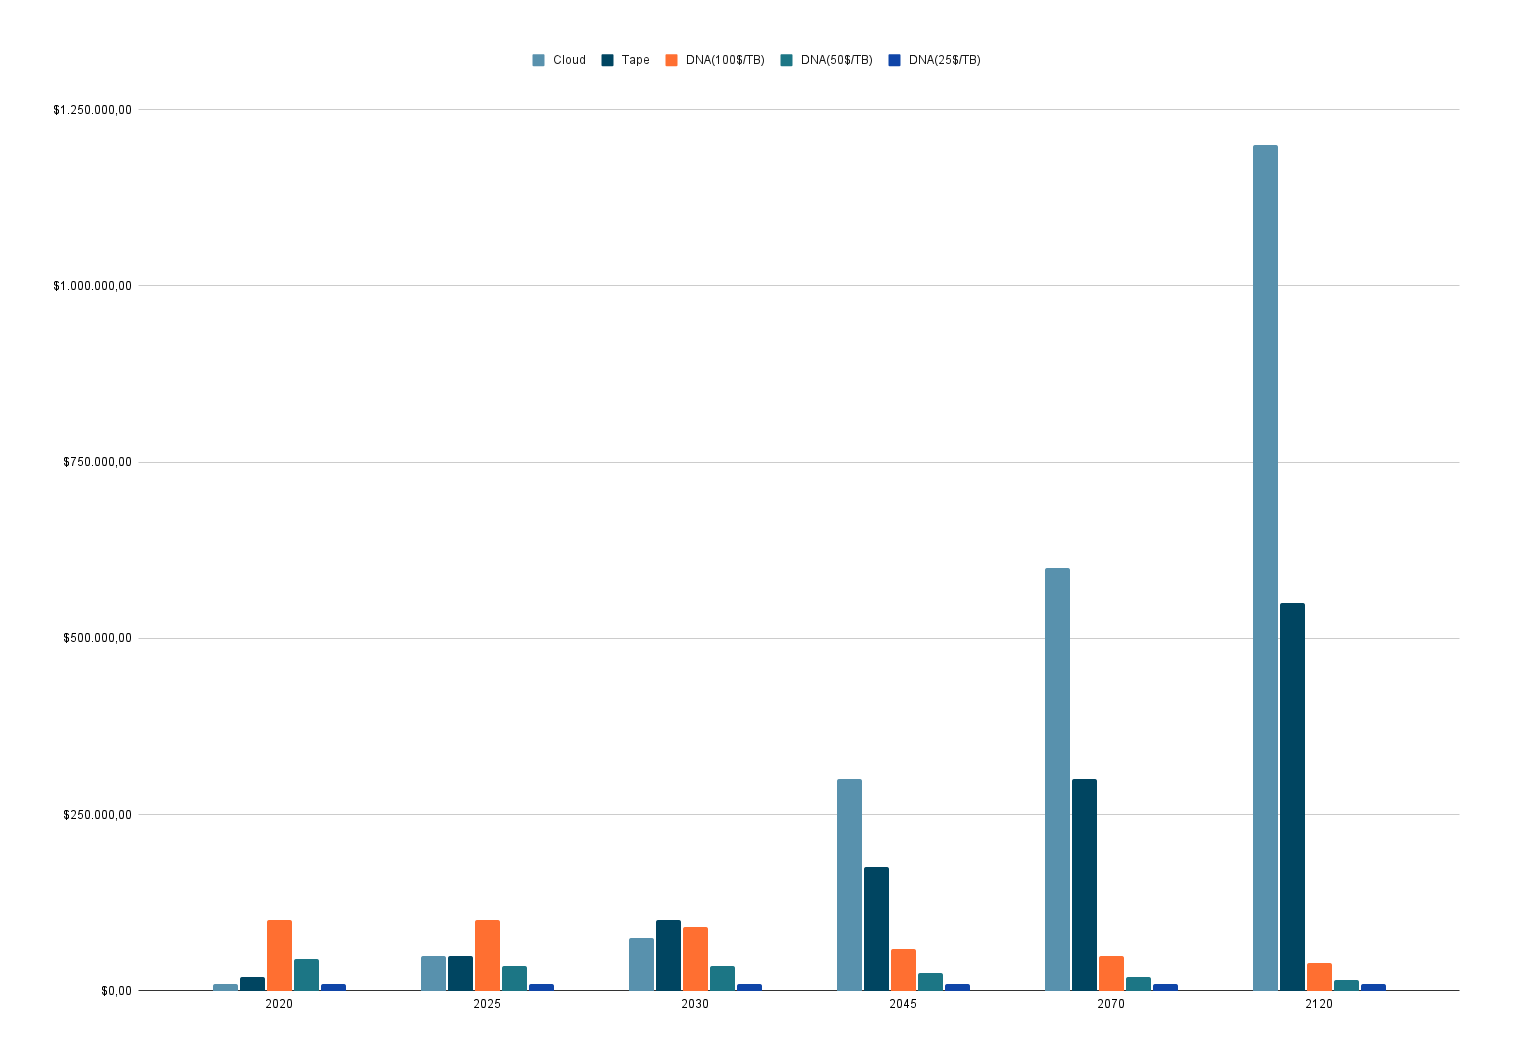
\includegraphics[width=\linewidth]{Figures/economicschart.png}
\caption{This is a chart that is showing the trend of the cost of the classic storage system versus the one that takes in
account of the cost of DNA during the time.
We can see the cloud is going to increase exponentially during this time this is due to the fact of the main idea of how
it works, the user needs to have access to their data at any time in a short amount of data. So the real competitor of
DNA storage is the Tape, for the explanation done in Kyders Law in the first section of the paper Tape and HDD are
following a log-like shape and the tech at some point will reach a bound. On the other side DNA storage is going
to decrease are predicted to decrease its cost this is due to the fact that, it is a sector in continuous expansion and
where research could take more consistent steps in the future to consolidate the techniques of encoding sequencing
and decoding of information.}
\label{fig:my_label9}
\end{figure*}
\section{Conclusion and future works}
Taking stock of the current situation. DNA data storage is a process that takes into account many small steps and each step is a brick to build this complicated process. Each of these steps requires a thorough study of various subjects and therefore the involvement of various experts in the field. Focusing on this point is important to understand the difficulty in scaling this type of project, as to date there is no figure able to cover all the various sectors and sciences to carry out the process. This slows down and greatly limits the process of developing this technology, as each step must be carried out by various figures.\
Taking a more specific example it can be said that two types of specialists collaborate, the engineers / mathematicians and the biologists / chemists for often the research done in this field by these figures do not go hand in hand creating constraints on both sides. In addition to today, no real solution has been found to the problem is still a field all in the research and improvement phase and this unfortunately does not attract many investors, who do not see an immediate economic implication.
While for the future, many papers are focusing on breaking down the limits of writing speed on the molecule that do not allow a large scale scalability of the storage system, given the long times.



\bibliography{ourbib}
\end{document} 